\documentclass[progress]{cmpreport}

\usepackage{rotating}
\usepackage{subfloat}
\usepackage{color}
\usepackage{pdfpages}
\usepackage{graphicx}

\title{Progress Report for AI for playing classical strategy games - Quoridor}

\author{Ace Shyjan}

\registration{100390438}
\supervisor{Dr Michal Mackiewicz}

\ccode{CMP-6013Y}

%%%%%%%%%%%%%%%%%%%%%%%%%%%%%%%%%%%%%%%%%%%%%%%%%%%%%%%%%%%%%%%%%%
\begin{document}
\section{Project Introduction}

\subsection{Motivation and Aim}
My motivation for this project comes from my love for board games and my interest in creating computer AI and this project allows me to combine these interests by building a game in which I can explore how AI makes decisions. Creating an efficient algorithm will be challenging due to Quoridor's dual objective nature of moving pawns and placing down fences; however, by using algorithms like Minimax or MCTS, I can explore strategic decision-making that balances both actions while considering the long-term consequences of each move. The project will be built in Godot which is a game engine I have had many years of experience in.

\subsection{Objectives}
My aim for this project is to create a fully functional Quoridor game that allows a player to compete against the computer. In addition to developing the core gameplay mechanics, I plan to explore and implement various AI algorithms, such as Minimax, Monte Carlo Tree Search, and possibly Neural Networks, to assess their effectiveness in making strategic decisions.
\begin{itemize}
    \item Create a working game of Quoridor against 2 players
    \item Create a computer AI using Minimax Algorithm
    \item Explore other potential algorithms such as MCTS, Neural Network, etc.
    \item Add multiplayer functionality between 2 devices (Extra)
\end{itemize}

\section{Progress Report}
Currently, based on the Gantt Chart [\ref{pplan}], I have started the coding stage and recently completed the design phase. The coding stage will be the longest, with the implementation of the algorithms being the most time-consuming part.

\subsection{Design and Planning}
The key areas of planning focused on the pre-game user interface, the board, fences, movement, and game loop. For the main menu, I created a list of possible options that the user would be able to navigate. Designing the board was straightforward, as it was simply an X × X grid of tiles, whereas designing the fences proved more challenging. I decided to use buttons to represent the fences, which were positioned at the centre of every 2 × 2 grid of tiles. This design was much simpler to implement than other potential ideas, such as a drag-and-drop mechanism.

\noindent For movement, I took inspiration from Chess, where available tiles are highlighted upon selection, and I planned to implement a similar feature. Regarding the game loop, I chose to have players click a "Confirm" button to lock in their move. This approach allows players to explore possible moves and strategise — for example, they can click on different fences to consider how their opponent might respond.

\subsection{Board Options}
I began by focusing on the main menu and game options. The options implemented so far include player name, colour, and board size. These settings have been integrated into the game itself, as shown in Figure \ref{fig:options}.

\subsection{TileButton}
The next step was to work on the actual board. I created a \texttt{TileButton} scene that inherits from Godot's Button class. I instantiated this button b × b times, where b represents the size of the board. The resulting board is shown in Figure~\ref{fig:board}.

\subsection{FenceButton}
The \texttt{FenceButton} class also inherits from the Button class. This class contains two panels to display horizontal and vertical fences. I instanced \((b-1)^2\) \texttt{FenceButtons} and offset them so that they appeared in the middle of a \(2 \times 2\) grid of \texttt{TileButtons}, as shown in Figure~\ref{fig:board}.

\noindent I configured a toggle button to switch between horizontal and vertical modes. When a \texttt{FenceButton} is pressed, it displays the corresponding fence panel, and upon clicking confirm, the fence is placed. After the fence is placed, the adjacent \texttt{FenceButtons} are disabled to prevent overlapping. This behaviour is shown in Figure~\ref{fig:fence_blocking_leap}, where the red buttons represent the disabled \texttt{FenceButtons}.  

\subsection{Tile and Fence Connections}
To separate the user interface from the game logic for future use, I created the \texttt{Fence} and \texttt{Tile} classes to store their connections and associated buttons. Each tile has a connection in each cardinal direction, and these are stored in a 1D array. Calculating the connections between tiles and fences uses the length of the board/fence grids.  

Another connection that needed to be handled is the one that is removed when a fence is placed. The \texttt{Fence} class stores this information in a 3D array, where the first and second elements correspond to the horizontal and vertical fences, respectively. The second depth of the array stores the two possible sets of connections that can be removed for that direction, and the third depth stores the actual two tiles that would lose their connection.  

\subsection{Board State}
I created a \texttt{BoardState} class, which can be used later for the DFS and AI algorithms, as it stores the current state of the board, including tile connections, current pawn positions, and fences.

\subsection{Pawn Spawning}
Once the tiles and fences were in place, I started to handle the pawn spawning and movement. I created a \texttt{Pawn} class, which inherits from Godot's Panel class. I made the pawn a white circle so that I could change the colour by updating the panel's modulate.  

\noindent During my first attempt at spawning the pawns, I placed two pawns: one at the top centre for Player 2, and one at the bottom centre for Player 1. However, when I reached the pawn movement stage, I changed how the pawns were spawned. Instead, I spawned a pawn on each tile for each player. This way, for pawn movement, I could simply hide and show the pawn as needed.

\subsection{Advanced Pawn Movement}
Now that every tile has a connection, proper pawn movement can be set up. I first disable all tiles on the board, and then enable all tile connections for the tile that the player's pawn is currently on. When a fence is placed, the tile connection is severed, as shown in Figure~\ref{fig:fence_placement}.

\subsubsection{Pawn Leaping}
One of the rules states that if two pawns are adjacent, a pawn can leap over another pawn, provided that there isn't a fence behind the pawn to be leaped, as shown in Figure~\ref{fig:pawn_leaping}. I achieved this by checking if one of the connections contains the enemy pawn. I then determine the cardinal direction of that tile and multiply it by 2 to get the leaped tile position, if there is a connection between the enemy pawn and the leaped tile. Another rule is that to prevent a pawn from being entrapped, if the pawn cannot leap, it can move to the enemy pawn's tile connections, as shown in Figure~\ref{fig:fence_blocking_leap}. To achieve this, if a fence is blocking the leaped tile, we then get the adjacent tiles of the enemy pawn's tile.

\subsection{Game Loop}
Once the movement was set, the last step was the game loop. I used a bit to store the current player, which allowed me to store both players' actions in arrays. After the player clicks confirm, the \texttt{current\_player} bit is flipped. The bit has an attached setter, which then resets the board and stores the moveable locations. Lastly, I implemented a win condition that runs a check every time a pawn is moved, to determine if the pawns are at their respective goal lines (top and bottom of the board).

\section{Progress Evaluation}

\subsection{Current Achievements}
So far, I have been working on the first objective: "Create a working game of Quoridor against 2 players.". The base game is nearly completed, with the illegal fence check being the last step before having a fully working game of Quoridor.

\subsection{Risk Analysis}
The biggest problem so far was figuring out how to implement fences both graphically and logically. After a while, I realised that it was best to separate the fence logic and use it to update the tile connections. Another issue that arose were invalid tile connections. The problem stemmed from mapping the \(2 \times 2\) \texttt{Tile Grid} with a single \texttt{Fence Button}, while also using the \texttt{board\_size}. This was resolved later after examining the underlying logic.  

\noindent A future concern will be optimising the AI and DFS, ensuring the efficient use of C\# and threading in order to perform the calculations in a shorter period of time. Another oversight is that the \texttt{BoardState} class stores references to the actual class itself, rather than the index of the position in the grid. This might be a problem in the future, as duplicating board states to simulate moves may cause issues such as overwriting data on the original board, which is something I will need to be careful of.

\subsection{Conclusion}
The next steps will be to implement the illegal fence check. This will require a depth-first search and will be written in C\#. This is the final step in completing the local multiplayer. Once that is finished, I can work on implementing the Minimax and MCTS algorithms. I will be modifying the \texttt{BoardState} to use indexes, rather than references, as mentioned before, to make the DFS and AI algorithm implementations easier.

\newpage
\appendix
\section{Appendix}
\begin{figure}[h]
    \centering
    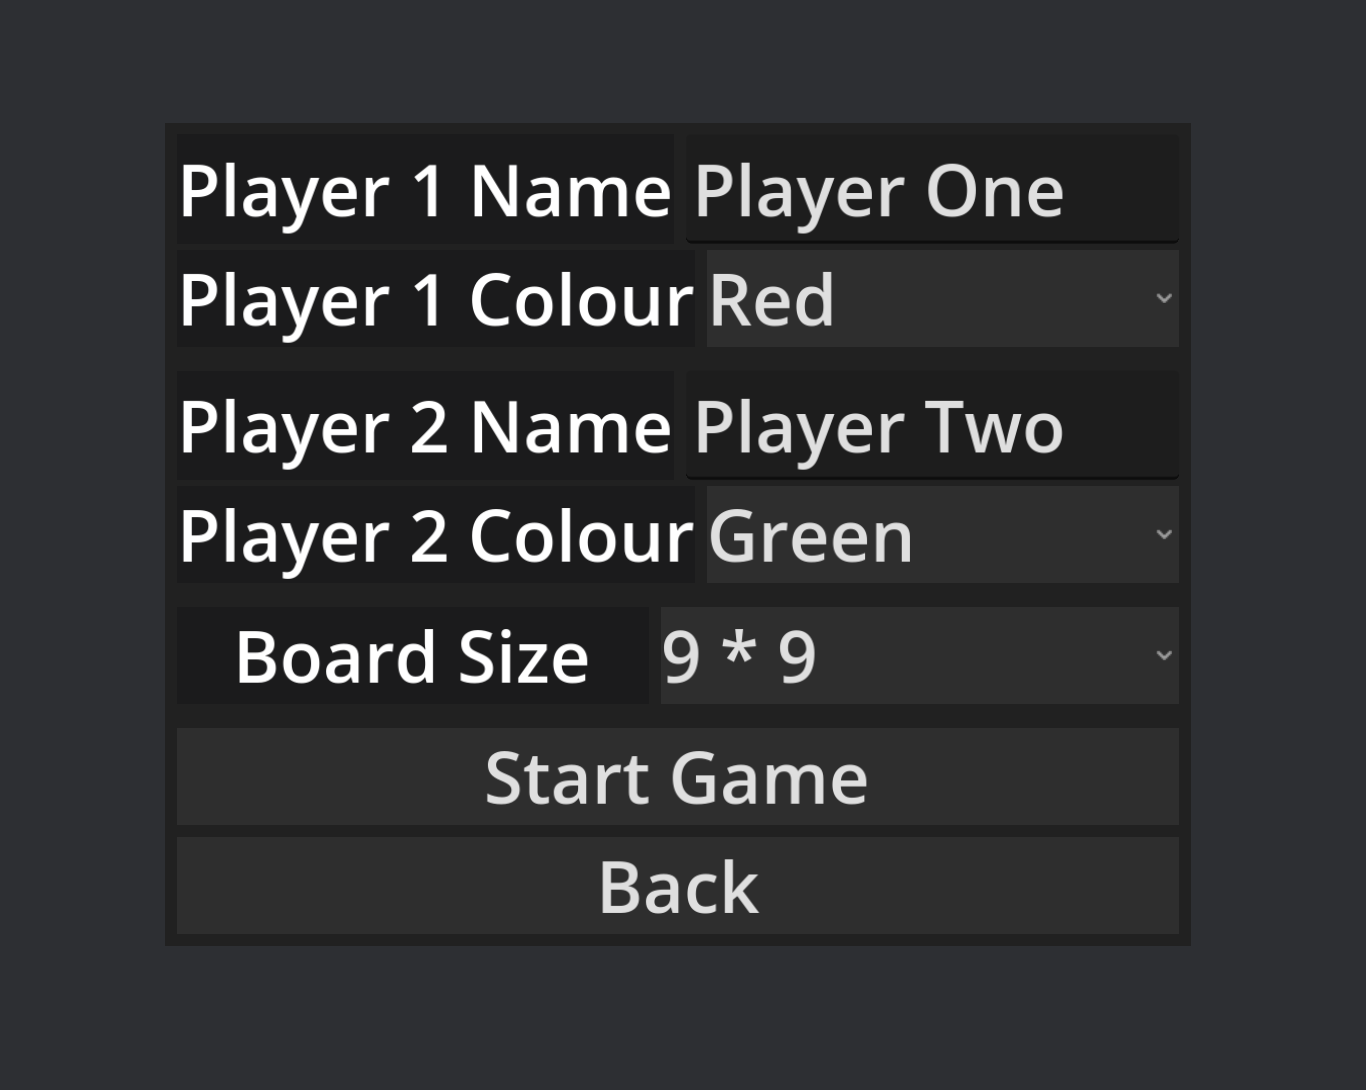
\includegraphics[width=0.4\textwidth]{images/board_options.png}
    \caption{Board Settings for local multiplayer.}
    \label{fig:options}
\end{figure}
\begin{figure}[h]
    \centering
    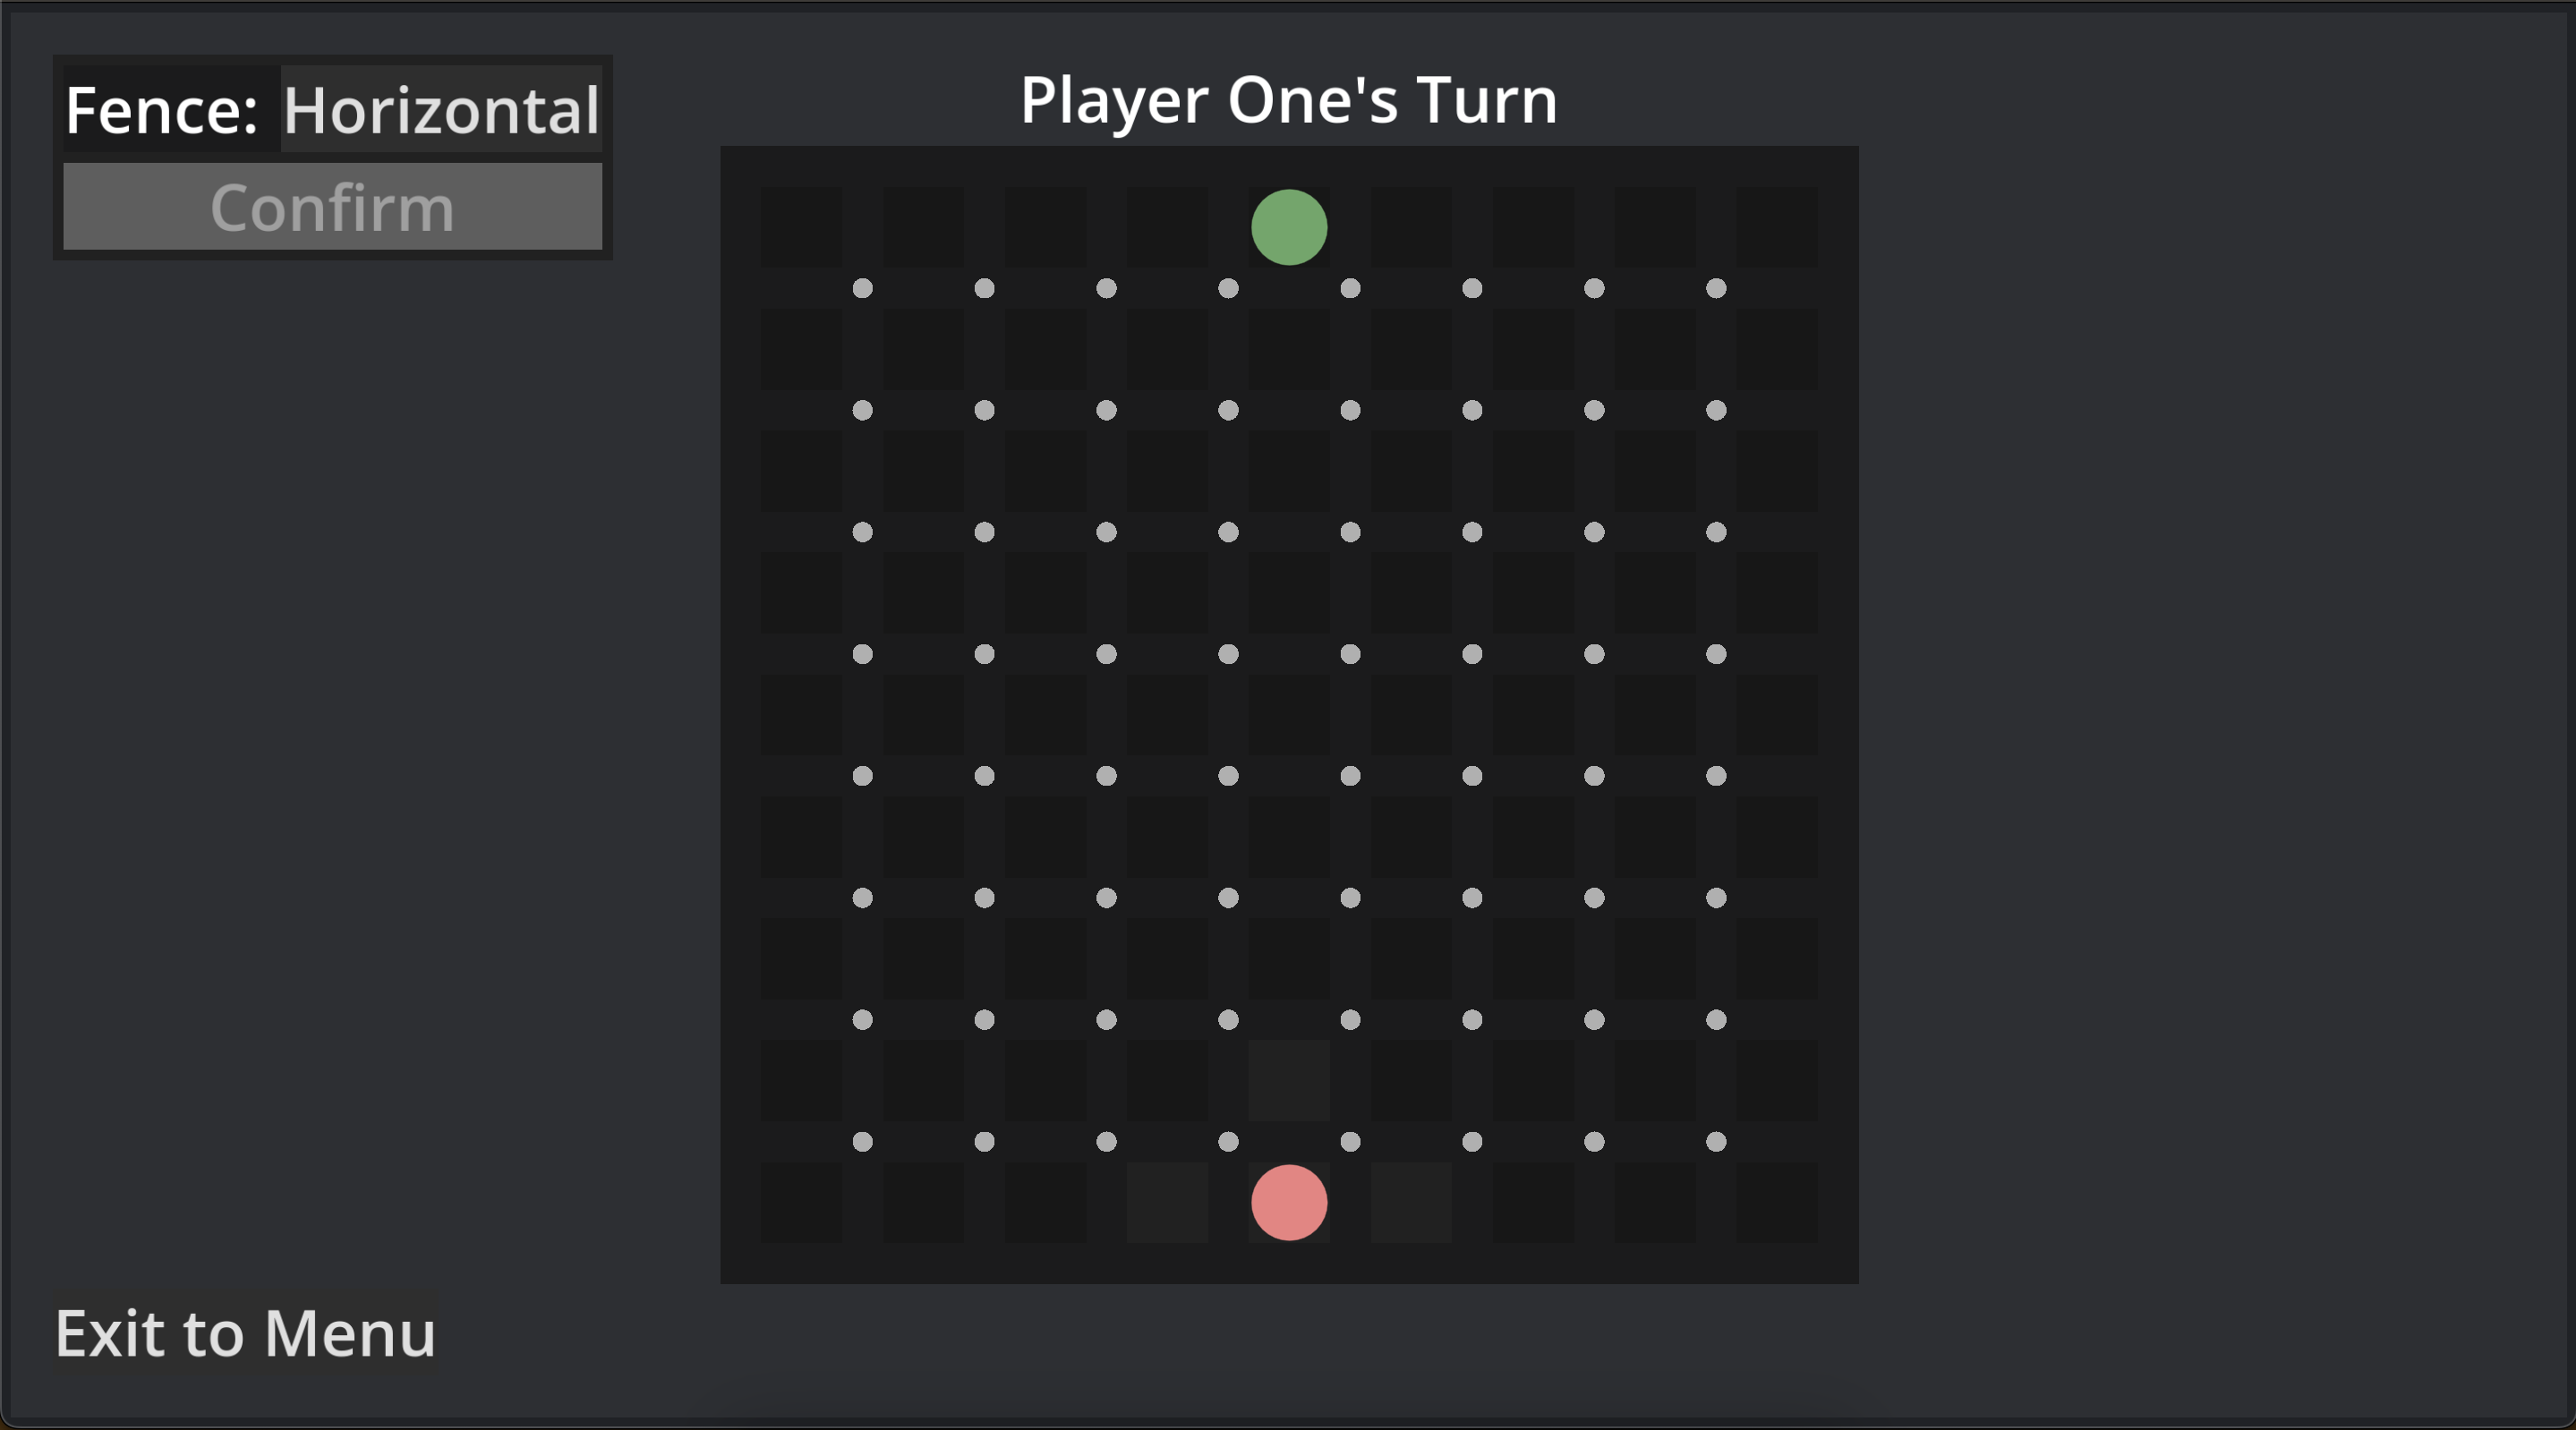
\includegraphics[width=0.6\textwidth]{images/current_board.png}
    \caption{Current Board.}
    \label{fig:board}
\end{figure}
\begin{figure}[h]
    \centering
    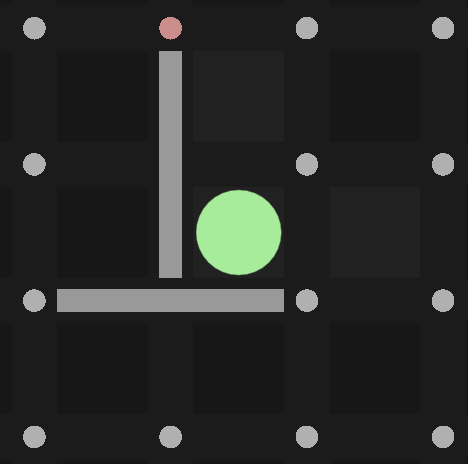
\includegraphics[width=0.6\textwidth]{images/fence_placement.png}
    \caption{Fence Placement.}
    \label{fig:fence_placement}
\end{figure}
\begin{figure}[h]   
    \centering
    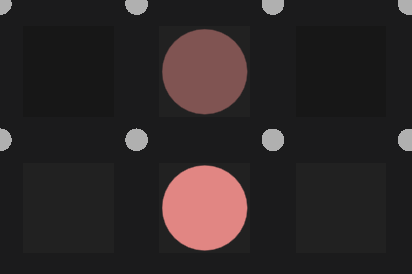
\includegraphics[width=0.6\textwidth]{images/pawn_movement.png}
    \caption{Pawn Movement.}
    \label{fig:pawn_movement}
\end{figure}
\begin{figure}[h]
    \centering
    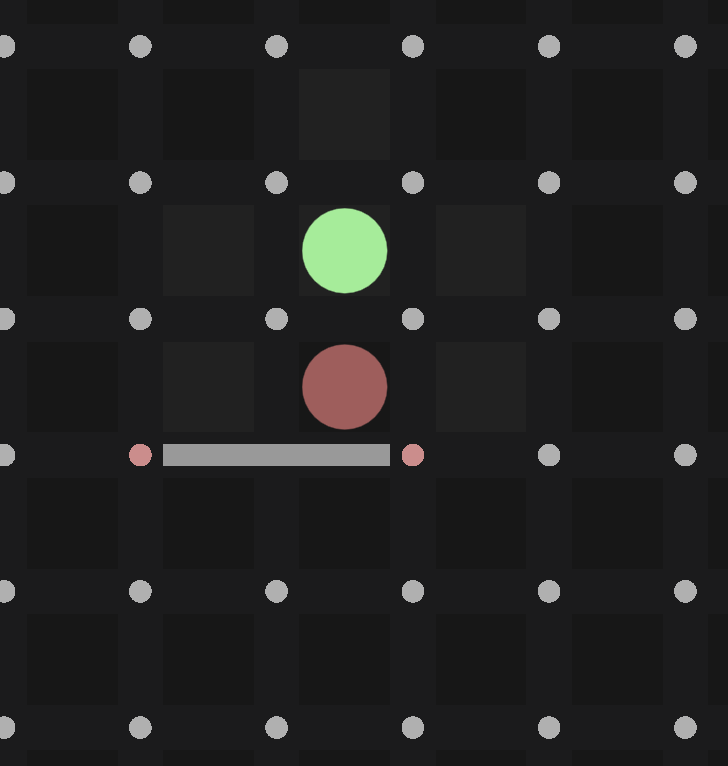
\includegraphics[width=0.6\textwidth]{images/fence_blocking_leap.png}
    \caption{A fence blocking a leap.}
    \label{fig:fence_blocking_leap}
\end{figure}
\begin{figure}[h]
    \centering
    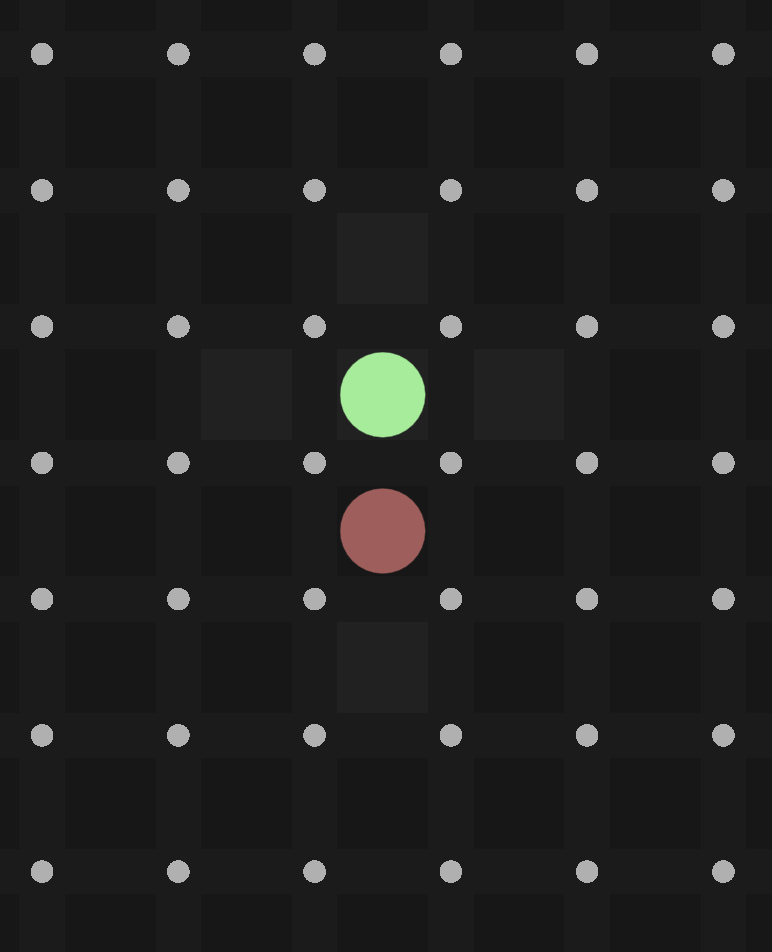
\includegraphics[width=0.6\textwidth]{images/pawn_leaping.png}
    \caption{Pawn Leaping.}
    \label{fig:pawn_leaping}
\end{figure}

\begin{cmpfigure}[htb]{Quoridor Development Gantt Chart \label{pplan}}
\begin{sideways}
\newganttchartelement{voidbar}{
voidbar/.style={
draw=black,
top color=black!25,
bottom color=black!23
}}
\begin{ganttchart}[x unit=0.4cm, y unit chart = 2.0cm, y unit title=0.5cm, title height=1.0, vgrid, title label font=\scriptsize,
canvas/.style={draw=black, dotted},
/pgfgantt/milestone left shift = 0,
/pgfgantt/milestone right shift = 0
]{4}{24}
\gantttitle{Project schedule for Quoridor development}{24} \\
\gantttitlelist{4,...,24}{1}\\
\ganttbar{Literature review}{4}{6}    \\  % elem1 
\ganttbar{Design phase}{7}{10}       \\  % elem2
\ganttbar{Coding}{9}{19}     \\  % elem3
\ganttbar{Testing and Refinement}{19}{22} \\  % elem4
\ganttbar{Final Adjustments}{22}{24}  \\ % elem5

% Links between the elements
\ganttlink{elem0}{elem1} 
\ganttlink{elem1}{elem2} 
\ganttlink{elem2}{elem3}
\ganttlink{elem3}{elem4} 
\end{ganttchart}
\end{sideways}
\end{cmpfigure}

\end{document}